\documentclass[main]{subfiles}

\begin{document}

% \resetcounters

\section{}

\subsection{Мотивация топологических методов}

Рассмотрим примеры задач, решаемых с помощью топологических методов.

\begin{theorem*}[о промежуточном значении функции]
	Пусть $ [a; b] \subset \R $, а $ f \colon [a; b] \to \R $ --- непрерывная функция,
	причем $ f(a) \Le f(b) $. Тогда для любой точки $ y \in [f(a); f(b)] $ существует такая точка
	$ x \in [a; b] $, что $ f(x) = y $.
\end{theorem*}


\begin{theorem*}[Бр\'{а}уэра]
	Пусть $ n \in \N $, а $ D \subset \R^n $ --- $ n $-мерный шар. Тогда для любой
	непрерывной функции $ f \colon D \to D $ существует такая точка $ x \in D $, что $ f(x) = x $.
\end{theorem*}


\begin{theorem*}[Б\'{о}рсука--\'{У}лама]
	Пусть $ n \in \N $, $ \S^n $ --- сфера в $ (n + 1) $-мерном протранстве,
	а $ f \colon \S^n \to \R^n $ --- непрерывная функция. Тогда существуют две такие
	диаметрально противоположные точки $ a, b \in \S^n $, что $ f(a) = f(b) $.
\end{theorem*}

\begin{example}
	Пусть $ n = 2 $, а $ f \colon (a, b) \mapsto (x, y) $, где $ x $ --- температура,
	а $ y $ --- давление в точке $ (a, b) $. Тогда существуют две диаметрально противоположные точки,
	где температура и давление совпадают.
\end{example}

\begin{theorem*}[о причесывании ежа]
	Пусть $ f \colon \S^2 \to \R^3 $ --- векторное поле, причем для любой
	точки $ x \in \S^2 $ вектор $ f(x) $ лежит в касательной плоскости к сфере в точке $ x $.
	Тогда существует такая точка $ x \in \S^2 $, что $ f(x) = 0 $.
\end{theorem*}

\begin{theorem*}[основная теорема алгебры]
	Всякий многочлен ненулевой степени имеет комплексный корень.
\end{theorem*}

\begin{theorem*}[\'{А}беля--Руфф\'{и}ни]
	Ни для какого натурального числа $ n \Gr 5 $ нельзя указать формулу,
	которая выражала бы корни любого уравнения степени $ n $ через его коэффициенты при помощи радикалов.
\end{theorem*}

\begin{remark}
	Для степени $ n = 3 $ есть формулы Кард\'{а}но, а для $ n = 4 $ --- формулы Ферр\'{а}ри.
\end{remark}

Все, кроме последнего примера, --- теоремы о существовании. Последний результат о несуществовании. В этом курсе будет
доказана теорема Брауэра. Многие рассуждения в доказательстве перечисленных утверждений можно свести к одной теореме:

\begin{restatable}{theorem}{ImageConnectivity}
	Образ связного пространства при непрерывном отображении является связным пространством.
\end{restatable}

В дальнейшем мы формализуем и конкретизируем это утверждение. В топологии требуется владеть техническими средствами
для доказательства фактов. Правдоподобные рассуждения могут приводить к неверным выводам.

\begin{example} <<Контринтуитивные>> результаты в топологии.
	\begin{itemize}
	\item Кривая Пеано: замощение квадрата непрерывной кривой, то есть
		существовании непрерывной сюръективной функции $ f \colon [0; 1] \to [0; 1]^2 $
	\item Кривая Вейерштрасса: существовании нигде не дифференцируемой непрервной функции.
	\item Определим $ C(f) $ как множество точек непрерывности функции $ f \colon \R \to \R $. Тогда существует такая
		функция $ f $, что $ C(f) = \R \wo \Q $, и не существует такая функция $ f $, что $ C(f) = \Q $.
	\end{itemize}
\end{example}

\subsection{Топологические пространства и открытые множества}

В любой науке основополагающим является понятие равенства двух объектов, поскольку именно оно определяет свойства,
по которым объекты могут различаться; эти свойства наука и изучает. Например, геометрия изучает свойства
геометрических фигур, инвариантные при движении. В алгебре есть понятие изоморфности групп, колец, полей и других
алгебраических структур. Топология, в отличие от геометрии, от метрических свойств абстрагируется, например, круг и
овал --- эквивалентные топологические пространства, хотя, скажем, круг и интервал --- нет. В алгебре понятие равенства
--- изоморфность. В топологии сходное значение имеет термин <<гомеоморфность>>. Дадим для начала нестрогие определения
основных понятий, используемых в курсе топологии.

\begin{definition}
	\emph{Топология $ \W $ на множестве $ T \neq \Emp $} --- это класс подмножеств множества $ T $,
	замкнутый относительно объединения. Иными словами, $\W$ --- топология на множестве $ T $,
	если существает такое множество $ B \ssq 2^T $,
	что $ \W = \Set{ \bigcup_{U \in \Nice{A}} U \mid \Nice{A} \ssq B } $.
\end{definition}

\begin{remark}
	Элементы множества $ B $ иногда называют окрестностями.
\end{remark}

\begin{definition}
	\emph{Топологическое пространство} --- это пара $ (T, \W) $, где $ \W $ --- топология на множестве $ T $.
\end{definition}

\begin{remark}
	Часто будем писать просто $ T $, называя его топологическим пространством. В этом случае имеется в виду, что на
	множестве $ T $ задана некоторая топология (либо она очевидна из контекста, либо не имеет большого значения).
\end{remark}

\begin{definition}
	Пусть $ (T, \W) $ --- топологическое пространство.
	Тогда элементы множества $ \W $ называются \emph{открытыми множествами}.
\end{definition}

\begin{definition}
	Пусть $ (T, \W) $ --- топологическое пространство.
	Тогда множество $ A \ssq T $ называется \emph{замкнутым}, если множество $ T \wo A $ открыто.
\end{definition}

\begin{example} Уже известные топологические пространства.
	\begin{itemize}
		\item Если $ T = \R $ и $ B = \Set{ (a, b) \subset \R \mid a < b } $,
			то элементы соответствующей топологии ---
			<<обычные>> открытые множества.
		\item Пусть $ n \in \N $, $ r > 0 $, $ x \in \R^n $ и $ B^n_r(x) $ --- $ n $-мерный шар радиуса $ r $
			с центром в точке $ x $.
			Тогда если $ T = \R^n $, а $ B = \Set{ B^n_r(x) \mid x \in \R^n; r > 0 } $, то соответствующая топология
			--- открытые множества в $ n $-мерном пространстве.
		\item Обобщение предыдущего примера. Можно считать, что
			$ B^n_r(x) = \Set{ x' \in \R^n \mid \mu(x, x') < r } $,
			где $ \mu $ --- произвольная метрика в $ \R^n $.
	\end{itemize}
\end{example}

Есть два способа определить, что заданное множество является открытым.

\begin{theorem} Пусть $ (T, \W) $ --- топологическое пространство,
	причем $ \W $ задается множеством $ B \ssq T $, и $ U \ssq T $. Тогда следующие условия эквивалентны:
	\begin{enumerate}
		\item существует такое множество $ \Nice{A} \ssq B $, что $ U = \bigcup_{W \in \Nice{A}} W $;
		\item для любой точки $ x \in U $ существует такое множество $ V \in B $, что $ x \in V $ и $ V \ssq U $.
	\end{enumerate}
\end{theorem}

\begin{proof} \leavevmode
	\begin{multiproof}
		\item[$\ft{1}{2}$] Раз $ U = \bigcup_{W \in \Nice{A}} W $, то для любой точки $ x \in U $ существует
			некоторое множество $ V \in \Nice{A} $, содержащее точку $ x $; более того, $ V \ssq U $.
			Так как $ \Nice{A} \ssq B $, то $ V \in B $. Таким образом, получаем требуемое.
		\item[$\ft{2}{1}$] Обозначим для каждой точки $ x \in U $ это множество через $ V_x $.
			Так как $ x \in V_x $ и $ V_x \ssq U $, то
			$ U = \bigcup_{x \in U} \Set{ x } \ssq \bigcup_{x \in U} V_x \ssq U $, откуда
			$ U = \bigcup_{x \in U} V_x $. Таким образом, зная, что $ V_x \in B $, остается положить
			$ \Nice{A} = \Set{ V_x \mid x \in U } \ssq B $.
	\end{multiproof}
\end{proof}

\begin{remark}
	По определению $ \W = \Set{ \bigcup_{W \in \Nice{A}} W \mid \Nice{A} \ssq B } $, откуда тривиально следует, что
	условие $(1)$ эквивалентно условию $ U \in \W $, то есть открытости множества $ U $.
\end{remark}

\begin{remark}
	В доказательстве $\ft{2}{1}$ используется аксиома выбора.
\end{remark}

\subsection{Гомеоморфизмы и непрерывность}

\begin{definition}
	Пусть $ (T_1, \W_1) $ и $ (T_2, \W_2) $ --- топологические пространства. Тогда:
	\begin{itemize}
		\item \emph{гомеоморфизмом топологических пространств} $ (T_1, \W_1) $ и $ (T_2, \W_2) $ называется такое
			взаимно однозначное отображение $ f \colon T_1 \to T_2 $, что для любого множества $ A \ssq T_1 $ верно
			$ A \in \W_1 \iaoi f(A) \in \W_2 $;
		\item если между двумя топологическими пространствами $ (T_1, \W_1) $ и $ (T_2, \W_2) $ существует
			гомеоморфизм, то они называются \emph{гомеоморфными}; в этом случае пишут
			$ (T_1, \W_1 ) \simeq (T_2, \W_2) $ или просто $ T_1 \simeq T_2 $.
	\end{itemize}
\end{definition}

\begin{example}
	Множество $ \R $ (со стандартной топологией, то есть с <<обычными>> открытыми множествами) гомеоморфно
	интервалу $ \left( -\frac{\pi}{2}; \frac{\pi}{2} \right) $, так как сушествует гомеоморфизм $ \arctg $
	(вскоре станет очевидно, почему это действительно гомеоморфизм).
\end{example}

Ослабив понятие гомеоморфизма, можно получить определения открытого и непрерывного отображения.

\begin{definition}
	Пусть $ (T_1, \W_1) $ и $ (T_2, \W_2) $ --- топологические пространства. Тогда отображение
	$ f \colon T_1 \to T_2 $ называется \emph{открытым}, если для любого $ U \in \W_1 $ верно $ f(U) \in \W_2 $.
\end{definition}

\begin{definition}
	Пусть $ (T_1, \W_1) $ и $ (T_2, \W_2) $ --- топологические пространства. Тогда отображение
	$ f \colon T_1 \to T_2 $ называется \emph{непрерывным}, если для любого $ V \in \W_2 $ верно
	$ f^{-1}(V) \in \W_1 $.
\end{definition}

\begin{remark}
	Данное определение непрерывности не противоречит интуитивным соображениям. Например,
	пусть $ T_1 = [a; b] $, а $ T_2 $ --- произвольное топологическое пространство. Назовем путем непрерывное
	отображение отрезка в пространство $ T_2 $ и рассмотрим некоторое открытое множество $ V \in \W_2 $. Тогда его
	прообразом будем объединение нескольких частей отрезка $ [a; b] $. Кажется вполне логичным, что эти куски,
	а значит, и весь прообраз, должны быть открытыми множествами.

	\begin{figure}[H]
		\centering 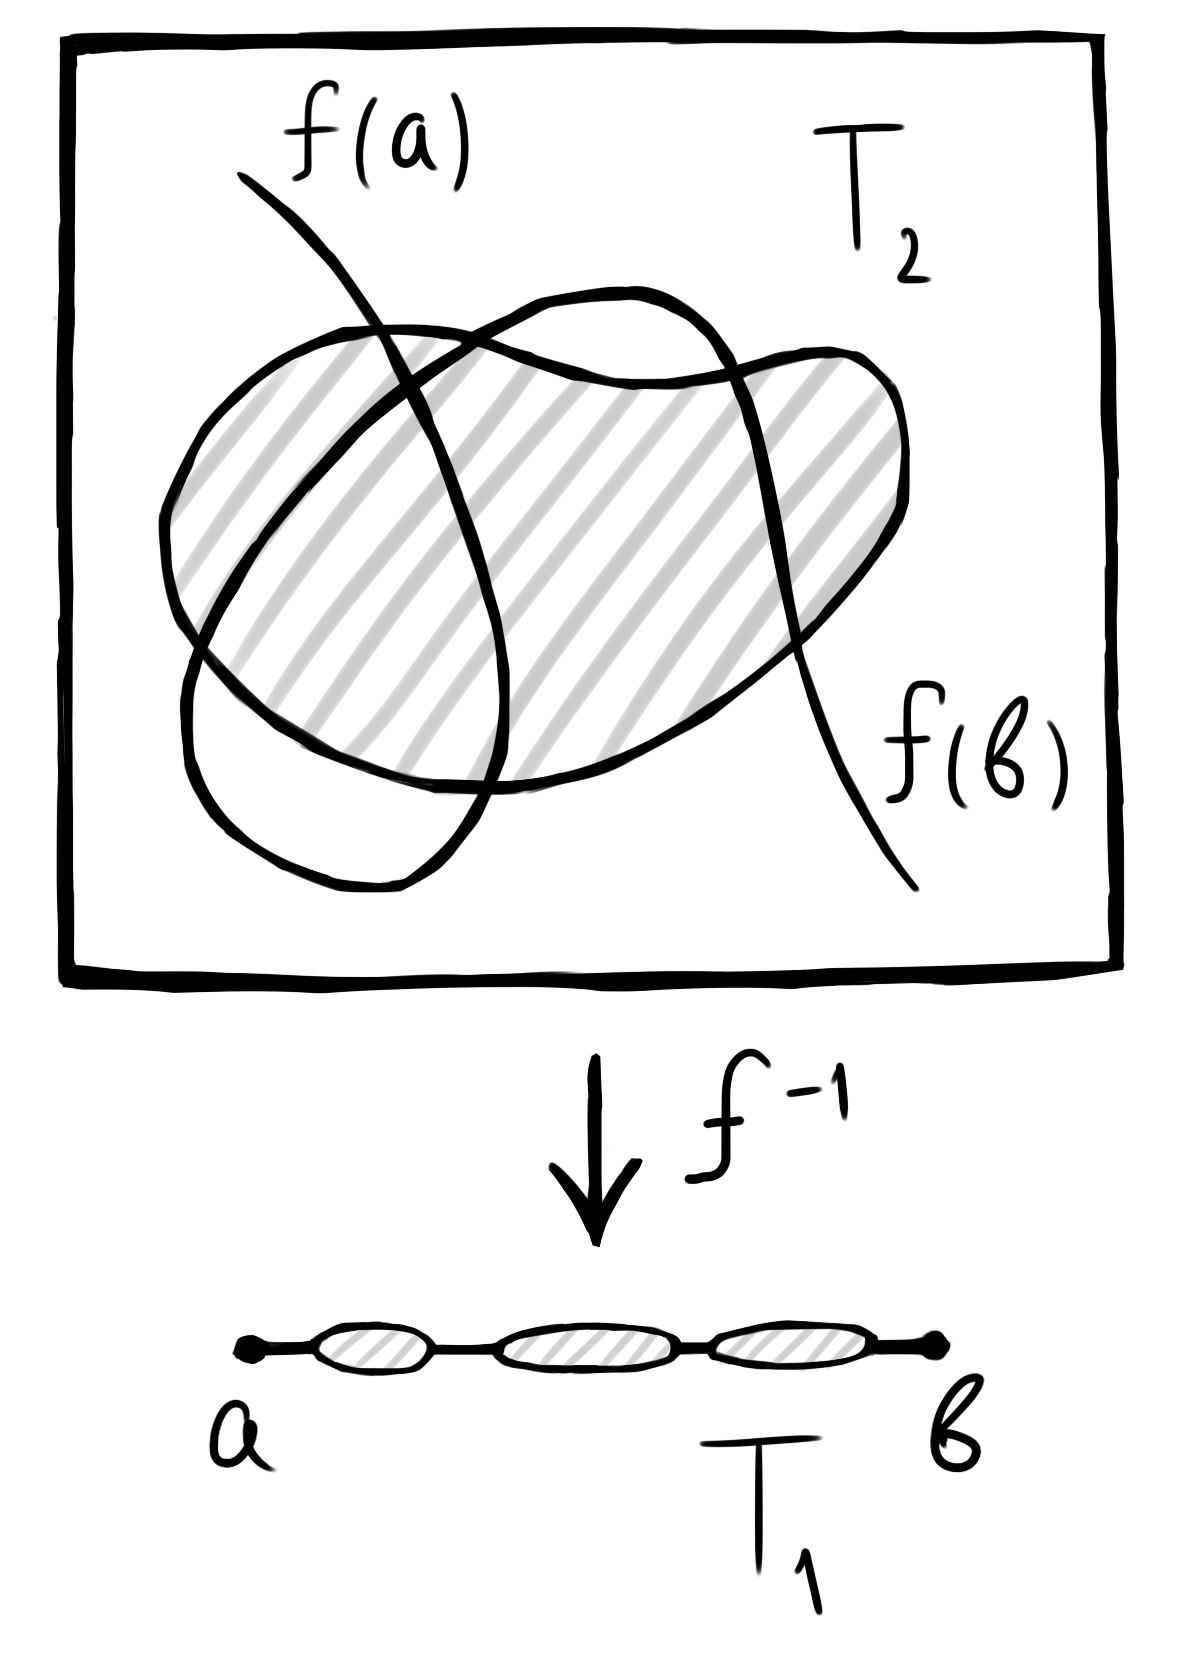
\includegraphics[width=0.5\textwidth]{continuity}
	\end{figure}
\end{remark}

\begin{restatable}{exercise}{ExcI}
	Вспомним определение непрерывности в точке, известное из курса математического анализа:
	отображение $ f \colon \R \to \R $ непрерывно в точке $ x \in \R $, если для любого $ \Eps > 0 $ существует такое
	число $ \delta > 0 $, что $ f(B_\delta (x)) \ssq B_\Eps(x) $. Докажите, что отображение $ f $ непрерывно по
	<<новому>> определению тогда и только тогда, когда оно непрерывно в каждой точке по <<старому>> определению.
\end{restatable}

\begin{remark}
	Пусть $ (T, \W) $ --- топологическое пространство. Окрестностью точки $ x \in T $ можно назвать как множество
	$ U \in \W $, содержащее точку $ x $, так и множество $ U \in B $, содержащее точку $ x $, если $ B $ задает
	топологию $ \W $. Это не определение, формально мы определим понятие окрестности позднее.
\end{remark}

Теперь дадим сразу четыре определения непрерывности отображения в точке. Позже мы докажем их эквивалентность,
но сначала воспользуемся ими, чтобы доказать, что отображение непрерывно тогда и только тогда,
когда оно непрерывно в каждой точке.

\begin{definition}
	Пусть $ (T_1, \W_1) $ и $ (T_2, \W_2) $ --- топологические пространства. Тогда отображение
	$ f \colon T_1 \to T_2 $ называется \emph{непрерывным в точке} $ x \in T_1 $, если выполнено одно из
	четырех условий:
	\begin{enumerate}
		\item для любой окрестности $ V \in B_2 $ точки $ f(x) $ существует
			такая окрестность $ U \in B_1 $ точки $ x $, что $ f(U) \ssq V $;
		\item для любой окрестности $ V \in B_2 $ точки $ f(x) $ существует
			такая окрестность $ U \in \W_1 $ точки $ x $, что $ f(U) \ssq V $;
		\item для любой окрестности $ V \in \W_2 $ точки $ f(x) $ существует
			такая окрестность $ U \in B_1 $ точки $ x $, что $ f(U) \ssq V $;
		\item для любой окрестности $ V \in \W_2 $ точки $ f(x) $ существует
			такая окрестность $ U \in \W_1 $ точки $ x $, что $ f(U) \ssq V $;
	\end{enumerate}
\end{definition}

\begin{theorem}
	Пусть $ (T_1, \W_1) $ и $ (T_2, \W_2) $ --- топологические пространства, и задано
	отображение $ f \colon T_1 \to T_2 $. Тогда отображение $ f $ является непрерывным $ \iaoi $
	отображение $ f $ является непрерывным в каждой точке $ x \in T_1 $.
\end{theorem}

\begin{proof} \leavevmode
	\begin{multiproof}
		\item[$\Then$] Рассмотрим точку $ x \in T_1 $ и окрестность $ V \in \W_2 $ точки $ f(x) $.
			Положим $ U = f^{-1}(V) $, тогда из непрерывности $ U \in \W_1 $, а из свойств пробраза $ x \in U $ и
			$ f(U) = f(f^{-1}(V)) \ssq V $, что и требовалось.
		\item[$\If$] Рассмотрим множество $ V \in \W_2 $ и произвольную точку $ x \in f^{-1}(V) $,
			тогда ее окрестностью будет некоторое множество $ U \in B_1 $, которое существует по определению
			непрерывности в точке. Значит, $ f(U) \ssq V $, откуда $ U \ssq f^{-1}(V) $. Согласно критерию
			$(2)$ открытости множества множество $ f^{-1}(V) $ открыто, что и требовалось.
	\end{multiproof}
\end{proof}

\begin{remark}
	После ознакомления со всеми определениями непрерывности, этой теоремой и упражнением становится ясно,
	что гомеоморфизм --- это непрерывное взаимно однозначное отображение, обратное к которому тоже непрерывно.
	Теперь действительно очевидно, что $ \arctg $ является гомеоморфизмом прямой и интервала.
\end{remark}

\end{document}
